\documentclass [12pt, a4paper]{article}

%Includes 
\usepackage[utf8]{inputenc}
\usepackage{graphicx}
\usepackage{subfig}
\usepackage[spanish]{babel}
\graphicspath{{images/}}
\usepackage{imakeidx}
\usepackage{enumerate}
\usepackage{listings} 

\usepackage{color}
\usepackage{listings}

\lstset{ %Coonfiguración para los códigos
	language=C++,                % choose the language of the code
	basicstyle=\footnotesize,       % the size of the fonts that are used for the code
	numbers=left,                   % where to put the line-numbers
	numberstyle=\footnotesize,      % the size of the fonts that are used for the line-numbers
	stepnumber=1,                   % the step between two line-numbers. If it is 1 each line will be numbered
	numbersep=5pt,                  % how far the line-numbers are from the code
	backgroundcolor=\color{white},  % choose the background color. You must add \usepackage{color}
	showspaces=false,               % show spaces adding particular underscores
	showstringspaces=false,         % underline spaces within strings
	showtabs=false,                 % show tabs within strings adding particular underscores
	frame=single,           % adds a frame around the code
	tabsize=2,          % sets default tabsize to 2 spaces
	captionpos=b,           % sets the caption-position to bottom
	breaklines=true,        % sets automatic line breaking
	breakatwhitespace=false,    % sets if automatic breaks should only happen at whitespace
	escapeinside={\%*}{*)}          % if you want to add a comment within your code
}
% Inicio de documento
\title{UNIVERSIDAD DE BUENOS AIRES\\FIUBA\\
	\vspace{10mm}
\includegraphics[scale=0.4]{fiuba}
	\vspace{5mm}\\66.20 Organización de Computadoras\\
	Trabajo práctico 0: Infraestructura básica\\1$^{er}$ cuatrimestre de 2018}

\author{ \textbf{ALUMNOS} 
	\vspace{5mm}\\
	\textbf{92454 ZARAGOZA, MARTIN}\\
	\textbf{92691 SIBIKOWSKI, NICOLAS}\\
	\textbf{91985 DUFAU, EZEQUIEL}\\
}
\date{}

\setlength{\parindent}{12pt}

\begin{document}

	
	\addtocontents{toc}{\hfill \textbf{Página} \par}
	
	\lstset{language=C}  
	\maketitle
	\clearpage
	\tableofcontents
	\clearpage
	\section{Introducción}
	Este documento representa la documentación técnica  del trabajo práctico 0, correspondiente a la materia \textbf{66.20 Organización de Computadoras}\\
	En el mismo se incluira el desarrollo de los siguientes puntos:
		\begin{itemize}
			\item Diseño e Implementación
			\item Compilación y ejecución del programa
			\item Corridas de prueba
			\item Código Fuente
		\end{itemize}
	\section{Diseño e Implementación} 
	Se desarrolló un programa que permite dibujar el conjunto de Julia, en lenguaje C.
	
	\subsection{Tipos de Datos Abstractos}
	Se diseñaron los siguientes TDAs:
	\subsubsection{\textbf{Pixel}}
		Define un punto en el plano complejo
	\begin{lstlisting}[frame=single]
typedef struct {
unsigned x;
unsigned y;
} Pixel;

typedef struct {
unsigned width;
unsigned height;  
} Dimension;

typedef Dimension Resolution;

void parseRes(char* str , Resolution* targetRes);

#endif
		
	\end{lstlisting}
	
	\vspace{5mm}
	\subsubsection{\textbf{Complex}}
		Define el TDA para manejar números complejos
	\begin{lstlisting}[frame=single]
typedef struct {
double re;
double im;
} Complex;

typedef struct {
double left;
double right;
double top;
double bottom;
} Boundaries;

Complex newCpx(double re , double im);

/** 
* Obtiene un numero complejo a partir de un string
*/
void parseCpx(char* str , Complex* targetCpx);

/**
* Obtiene la raiz cuadrada de un complejo
*/
Complex pow2Cpx(Complex* value);

Complex addCpx(Complex* first , Complex* second);

/** 
* Obtiene el modulo de un valor complejo 
  (distancia respecto al origen).
*/
double modCpx(Complex* value);

/** 
* Calcula los limites del plano complejo 
   (el rectangulo a mapear del plano complejo).
* Dimension dim - Tamano del plano complejo
* Complex center - Valor de centro EN EL plano
*/
Boundaries getBoundaries(Complex* dim , Complex* center);

#endif

	\end{lstlisting}
	
\subsubsection{\textbf{Arguments}}
Define una estructura que permite manejar los parámetros del programa
\begin{lstlisting}[frame=single]
#include "pixel.h"
#include "complex.h"

typedef struct {
Resolution resolution;  // resolucion de imagen
Complex center;         // centro del plano complejo
Complex cpxSize;        // tamano del plano complejo
Complex seed;           // semilla disparadora
char* outfile;          // archivo de salida
} Arguments;

Arguments parseArgs(int argc, char** args);

#endif

\end{lstlisting}
	
\subsection{Formate PGM}
	El formato utilizado para generar la imagen es el PGM. En sus especificaciones establece que ninguna linea debe tener más de 70 caracteres.\\Debido a esto se tomó la decisión de que el programa genere el número óptimo de caracteres que debe tener cada linea en el archivo. El número máximo de cada valor es 255 aproximadamente 3 caracteres, teniendo en cuenta los 70 caracteres por línea el máximo de valores es 16. Su funcionamiento se puede ver en el siguiente código 
	
	\begin{lstlisting}[frame=single]
unsigned getOptIndex(unsigned itemCount) {
	unsigned idx = 16;
	while(itemCount % idx-- > 0);
	return idx + 1;
}
	\end{lstlisting}
	\vspace{5mm} Donde itemCount sale de hacer
	\begin{lstlisting}[frame=single]
itemCount = resolution.width * resolution.height;
	\end{lstlisting}	
	\clearpage
	\section{Compilación y ejecución del programa}
	
	Utilizamos el programa GXemul para simular un entorno de desarrollo. El mismo consta de una máquina MIPS corriendo una versión del sistema operativo BSD. Debido a esto, el compilador utilizado utilizado es el que trae instalada la imagen provista por la cátedra. El mismo es el \textbf{(GCC) 3.3.3 (NetBSD nb3 20040520)}
	\\\\
	\subsection{Compilación}
	Para facilitar el proceso de compilación, programamos un Makefile, seteando las opciones correspondientes. Se debe ejecutar make en el directorio raiz del proyecto y el programa queda compilado. Se genera un ejecutable llamado app
	\subsection{Ejecución}
	Se debe ejecutar\\
	./app.exe [OPCIONES]\\
	
	\textbf{Opciones}:\\
	-r, o --resolution, permite cambiar la resolución de la imagen generada. El valor por defecto será de 640x480 puntos.\\\\
	-c, o --center, para especificar las coordenadas correspondientes al punto central de la porción del plano complejo dibujada, expresado en forma binómica (i.e. a+bi). Por defecto usaremos 0+0i.\\\\
	-w, o --width, especifica el ancho de la región del plano complejo que estamos por dibujar. Valor por defecto: 2.\\\\
	-H, o --height, sirve, en forma similar, para especificar el alto del rectángulo a dibujar. Valor por defecto: 2.\\\\
	-s, o --seed, para configurar el valor complejo de la semilla usada para generar el fractal. Valor por defecto: -0.726895347709114071439+0.188887129043845954792i.\\\\
	-o, o --output, permite colocar la imagen de salida, (en formato PGM [6]) en el archivo pasado como argumento; o por salida estándar -cout- si el argumento es “-”.\\\\
	
	
	\section{Corridas de prueba}
	\subsection{Valores por defecto}
	Se generó un dibujo usando los valores por defecto, barriendo la región rectangular del plano comprendida entre los vértices -2+2i y+2-2i.	La validación fue visual. Comparando contra un dibujo patrón disponible en el enunciado.
	
	\paragraph{Comando ejecutado: tp0 -o uno.pgm }
	
	Resultado de la prueba:
	\begin{figure}[h]
		\centering
		\subfloat[nuestro programa]{
			\label{f:nuestro}
			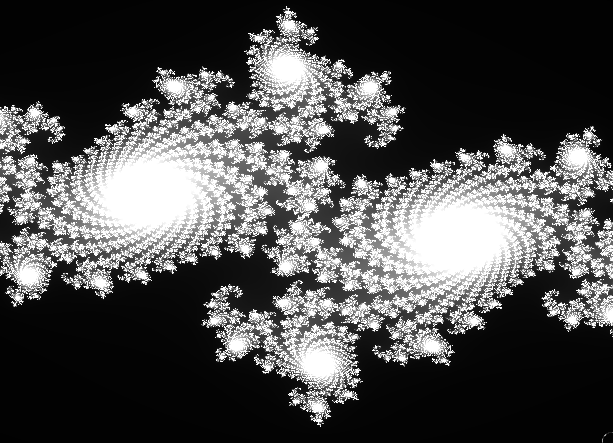
\includegraphics[width=0.3\textwidth]{uno.png}}
		\subfloat[trabajo práctico]{
			\label{f:tp}
			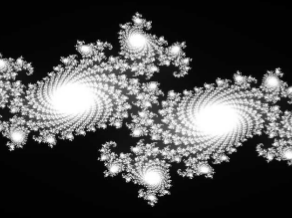
\includegraphics[width=0.3\textwidth]{unoTp}}
		\caption{Comparación entre imagen generada por el enunciado del tp, y nuestro programa}
		\label{f:comparacion1}
	\end{figure}
	\subsection{Zoom en región}
	Hacemos zoom sobre la región centrada en 0.282-0.007i, usando un
	rectángulo de 0.005 unidades de lado.
	
	\paragraph{Comando ejecutado: tp0 -c 0.282-0.007i -w 0.005 -H 0.005 -o dos.pgm}
	
	Resultado de la prueba:
	\begin{figure}[h]
		\centering
		\subfloat[nuestro programa]{
			\label{f:nuestro}
			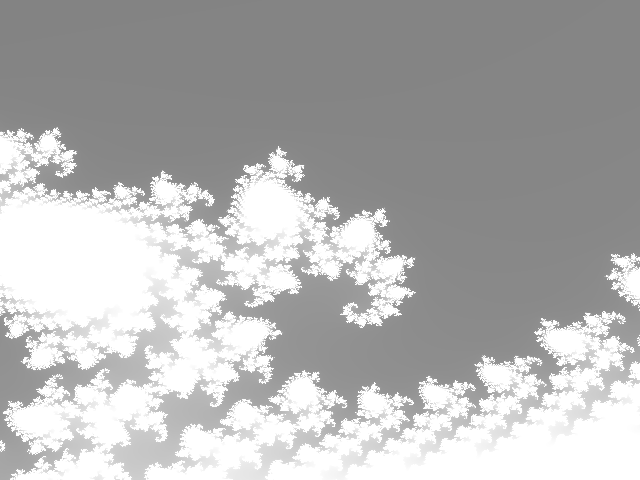
\includegraphics[width=0.3\textwidth]{dos}}
		\subfloat[enunciado del trabajo práctico]{
			\label{f:tp}
			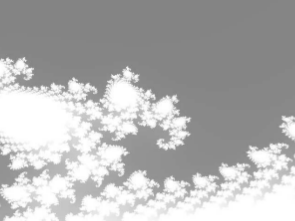
\includegraphics[width=0.3\textwidth]{dosTp}}
		\caption{Comparación entre la imagen generada por el enunciado del tp, y nuestro programa}
		\label{f:comparacion2}
	\end{figure}

	\subsection{Modificación de la semilla}
	En esta prueba vamos a modificar la semilla utilizando el comando -s. Apoyandonos mediante otra implementación del Algoritmo de Julia, vamos a comparar la imagen generada por nuestro programa coon la generada por la otra implementación. La implementación de Julia la obtuvimos en https://www.wolframalpha.com/juliaset.html
	Utilizamos la semilla  -0.742+0.1i.
	\\
	Ejecutamos: ./tp -o salida.pgm -s -0.742+0.1i\\
	Resultado de la prueba:
		\begin{figure}[h]
		\centering
		\subfloat[nuestro programa]{
			\label{f:nuestro2}
			
\includegraphics[width=0.3\textwidth]{cuatro}}
		\subfloat[Wolframalpha]{
			\label{f:tp}
			
\includegraphics[width=0.3\textwidth]{cuatroWolf}}
		\caption{Comparación entre otra implementación del algoritmo de Julia y nuestro programa}
		\label{f:comparacion3}
	\end{figure}

	\subsection{Movimiento del centro}
	En esta prueba vamos a generar cuatro imagenes(una para cada cuadrante) de la imagen utilizada en la prueba de valores por defecto.
	
			\begin{figure}[h]
		\centering
		\subfloat[./tp -c -0.5+0.5i]{
			\label{f:supizq}
			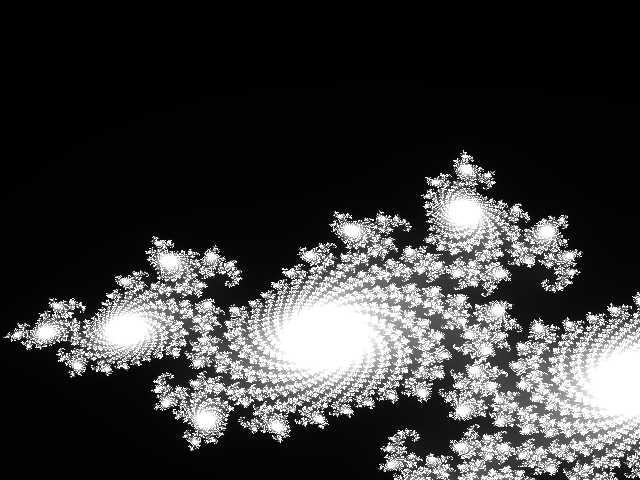
\includegraphics[width=0.3\textwidth]{supizq}}
		\subfloat[./tp -c 0.5+0.5i]{
			\label{f:supder}
			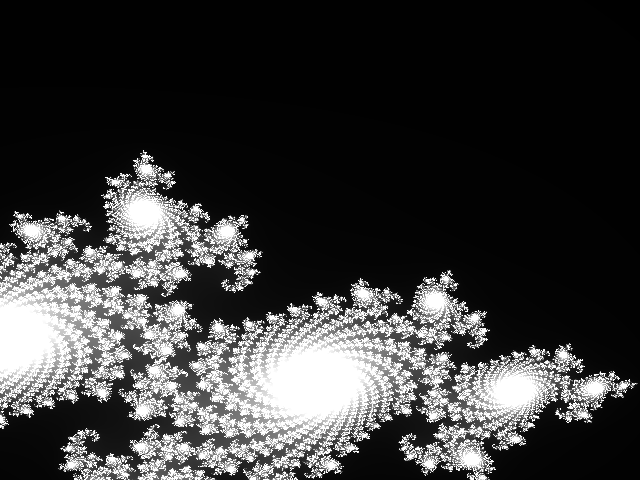
\includegraphics[width=0.3\textwidth]{supder}}
		\\ \subfloat[./tp -c -0.5-0.5i]{
			\label{f:infizq}
			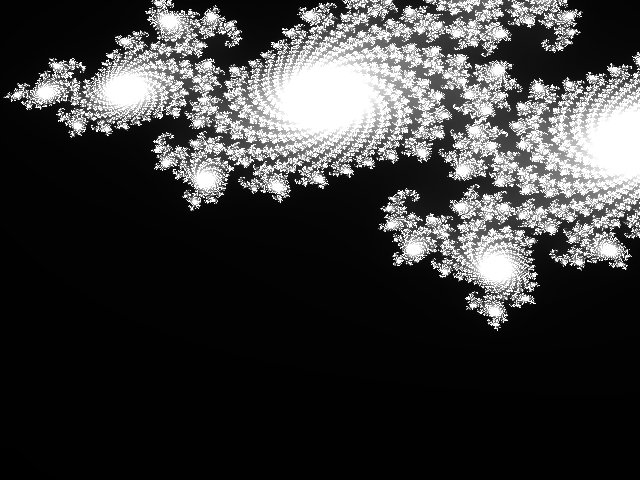
\includegraphics[width=0.3\textwidth]{infizq}}
		\subfloat[./tp -c 0.5-0.5i]{
			\label{f:infder}
			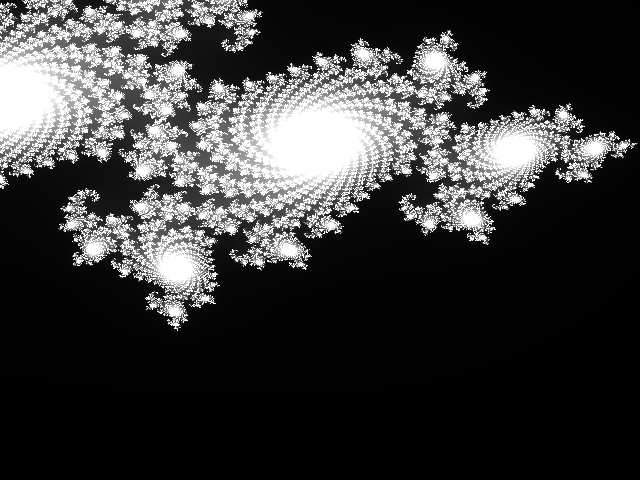
\includegraphics[width=0.3\textwidth]{infder}}
		\caption{Diferentes imagenes que permiten observar como se fue moviendo el centro según cada situación}
		\label{f:comparacion3}
	\end{figure} 
\subsection{Modificación de la resolución}
En esta prueba se modificará la resolución de la pantalla a 200*200 px. utilizando el comando -r
\\
Prueba ejecutada
Ejecutamos: ./tp -o salida.pgm -r 200*200\\

	\begin{figure}[h]
	\centering
	\subfloat[Resolución del archivo creado]{
		\label{f:resolucion}
		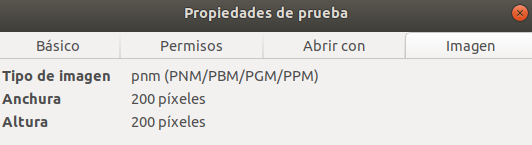
\includegraphics[width=\textwidth]{cinco}}
	\\\subfloat[Imagen creada]{
		\label{f:imgcuadrada}
		
\includegraphics[width=0.3\textwidth]{cincoimg}}
	\caption{Resultado de la prueba}
	\label{result5}
\end{figure}
	\clearpage
	\section{Código fuente}
	\paragraph{En esta sección incluiremos el código fuente de nuestra aplicación}
	{. }
	\lstinputlisting[language=C,caption=julia.c]{../src/julia.c}
	\lstinputlisting[language=C,caption=app.c]{../src/app.c}
	\lstinputlisting[language=C,caption=args.c]{../src/args.c}
	\lstinputlisting[language=C,caption=pixel.c]{../src/pixel.c}
	
\end{document}
